\documentclass{article}

\title{Assignment 7\\\normalsize{Advanced Programming}}
\author{Jordi Riemens\\Thomas Churchman}

\usepackage[utf8]{inputenc}
\usepackage{listings}
\lstset{basicstyle=\ttfamily}

\usepackage{graphicx}
\graphicspath{ {images/} }

\begin{document}
	\maketitle
	
	\section{Canceling tasks}
	We wanted to implement a method of gracefully canceling a task.
	For example, when working on the \emph{Manage proposal} task, a user might wish to cancel managing the proposal.
	We have attempted to include a cancellation action, but have not been able to get this to work nicely with the workflow framework.
	We tried returning various values, such as \lstinline|return ()|, \lstinline|throw "Cancel"|, and have tried changing the return type, as well as ending with an interaction task (\lstinline|viewInformation "Success" [] "Cancelled"|), but these either do not achieve the desired effect, or simply crash the iTasks GUI.
	In the current version 2017-11-08 nightly version of iTasks, the ``Close"-button supplied by the iTasks worklist framework also crashes the GUI.
	As such, we assume there is a bug in the current iTasks version that prevents such buttons from working as intended.
	
	\section{Appointment creation and parallel tasks}
	When an appointment is created (either from \emph{Make appointments} or from scheduling from a \emph{Manage proposal} task), a parallel task is detached.
	The task waits until the appointment start time, and then launches in parallel one task per participant to view the appointment.
	These tasks wait until the appointment end time and then finish.
	The tasks as detached, and not embedded, as a parallel task launched from a transient workflow is stopped once the transient workflow is closed.
	
	\newpage
	\appendix
	\section{Screenshots}
	
	\begin{figure}[h!]
		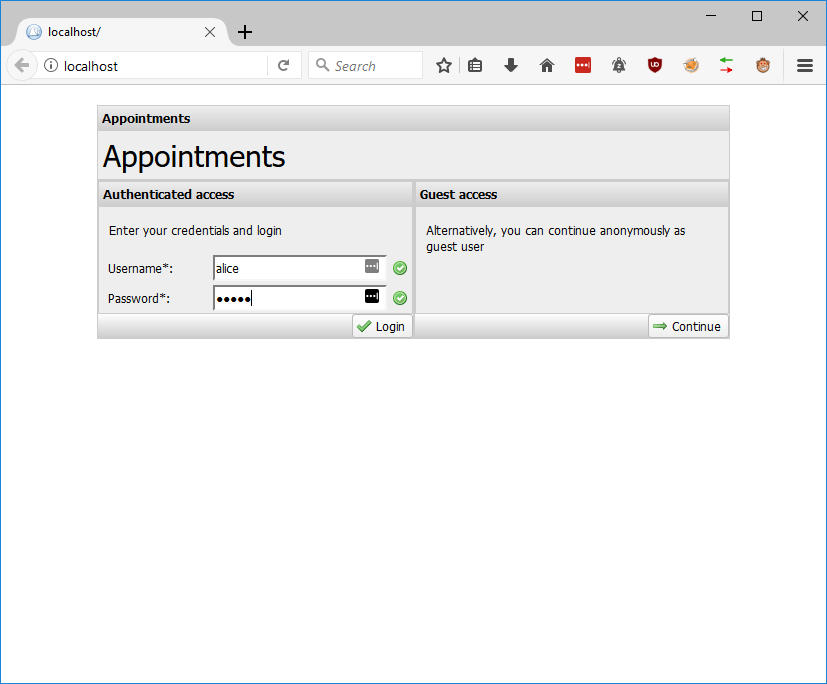
\includegraphics[width=\textwidth]{01_login}
		\caption{Logging in}
	\end{figure}
	
	\begin{figure}[h!]
		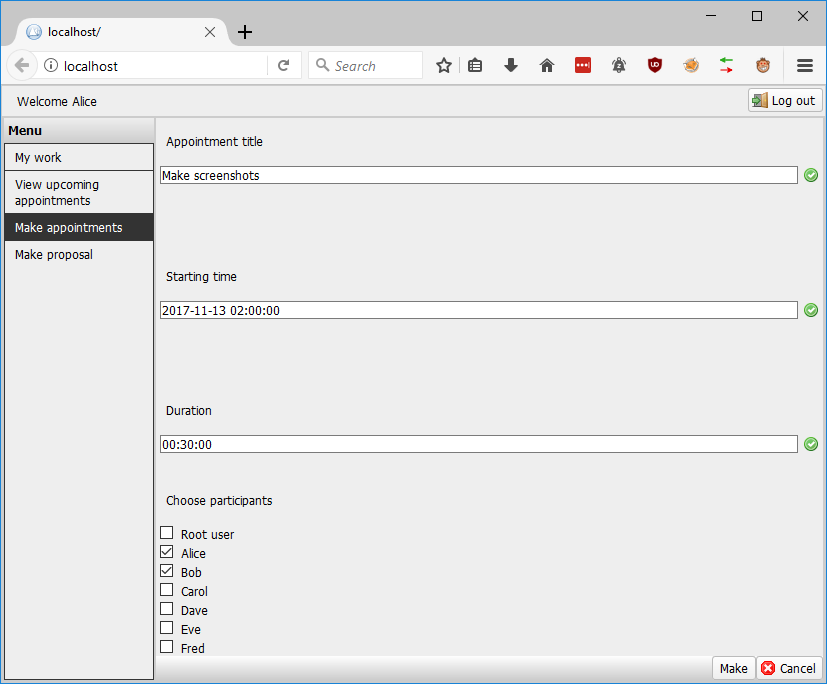
\includegraphics[width=\textwidth]{02_make_appointment}
		\caption{Making an appointment}
	\end{figure}
	
	\begin{figure}[h!]
		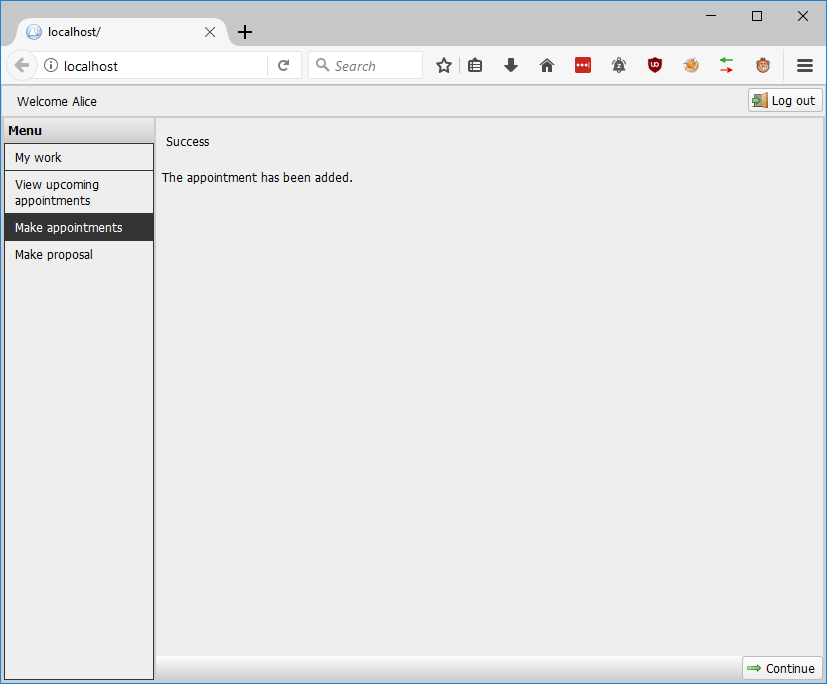
\includegraphics[width=\textwidth]{03_appointment_added}
		\caption{Appointment added}
	\end{figure}
	
	\begin{figure}[h!]
		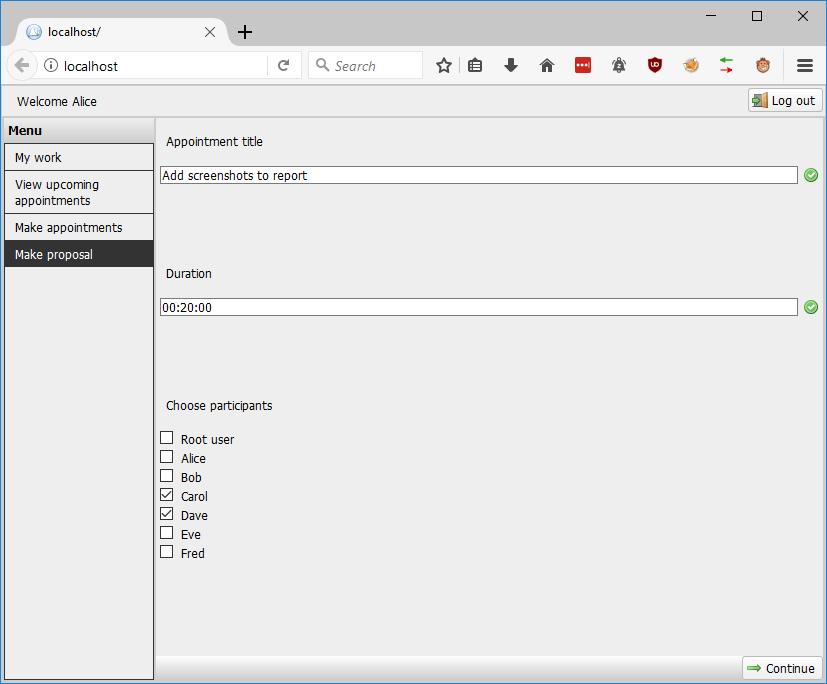
\includegraphics[width=\textwidth]{04_make_proposal}
		\caption{Proposing an appointment}
	\end{figure}
	
	\begin{figure}[h!]
		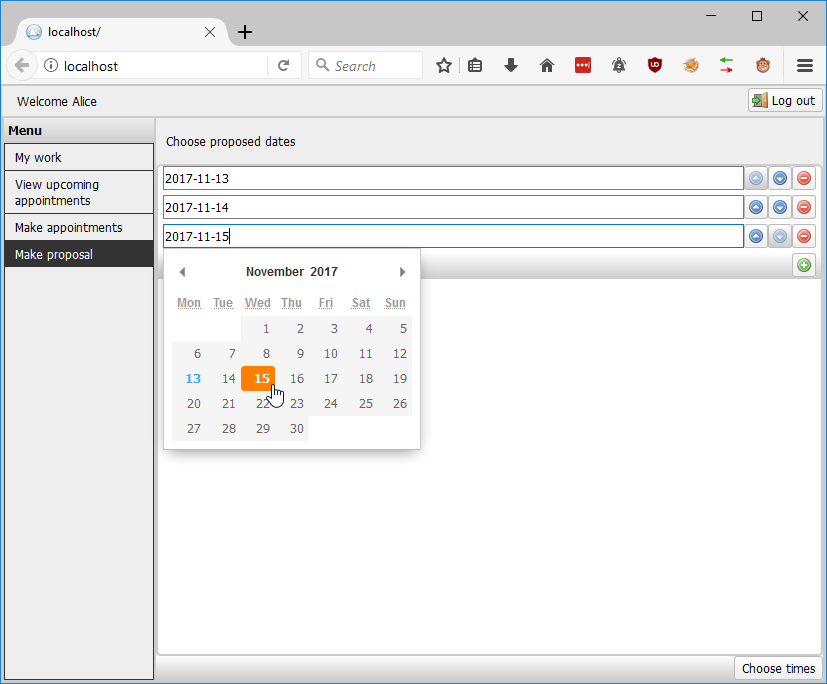
\includegraphics[width=\textwidth]{05_make_proposal_choose_dates}
		\caption{Proposing an appointment: choose dates}
	\end{figure}
	
	\begin{figure}[h!]
		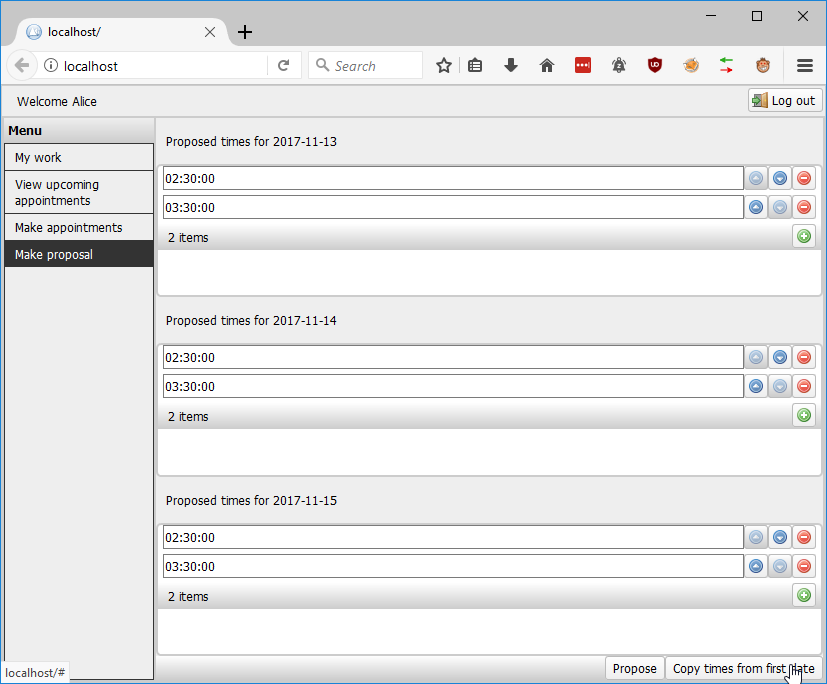
\includegraphics[width=\textwidth]{06_make_proposal_choose_times}
		\caption{Proposing an appointment: choose times}
	\end{figure}
	
	\begin{figure}[h!]
		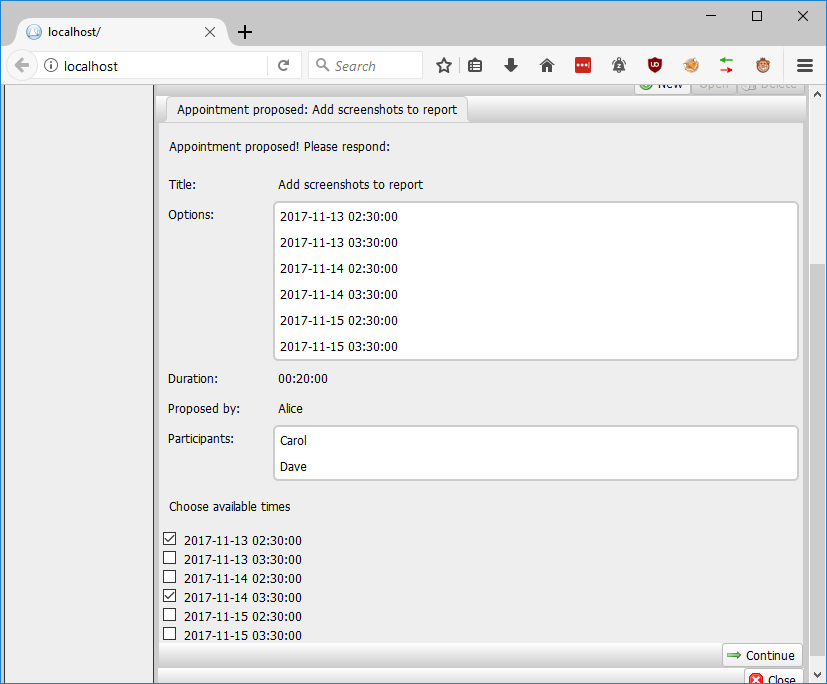
\includegraphics[width=\textwidth]{07_dave_choose_proposal_date_times}
		\caption{Viewing the appointment invitation: choose available dates and times}
	\end{figure}
	
	\begin{figure}[h!]
		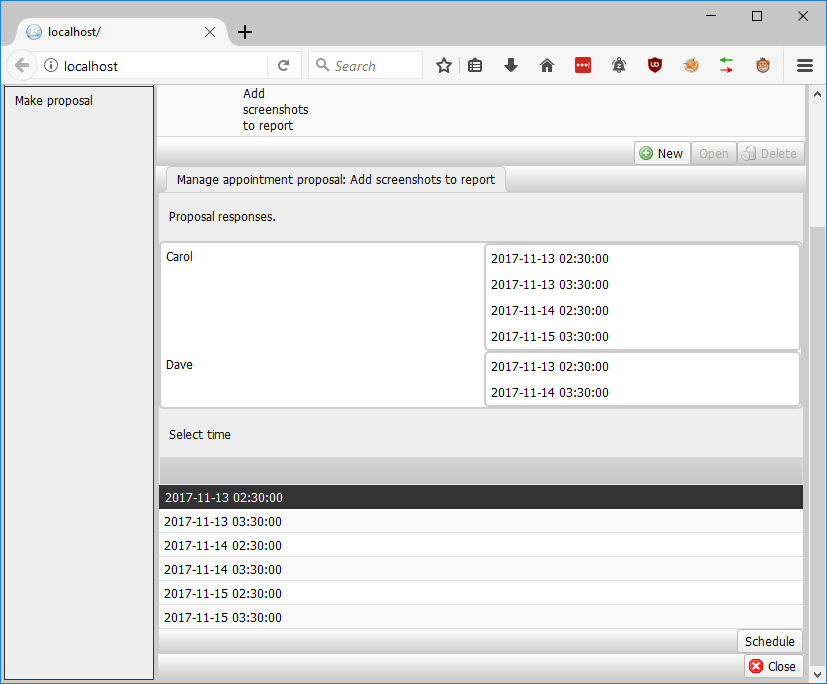
\includegraphics[width=\textwidth]{08_manage_proposal}
		\caption{Managing the proposal: see responses and schedule}
	\end{figure}
	
	\begin{figure}[h!]
		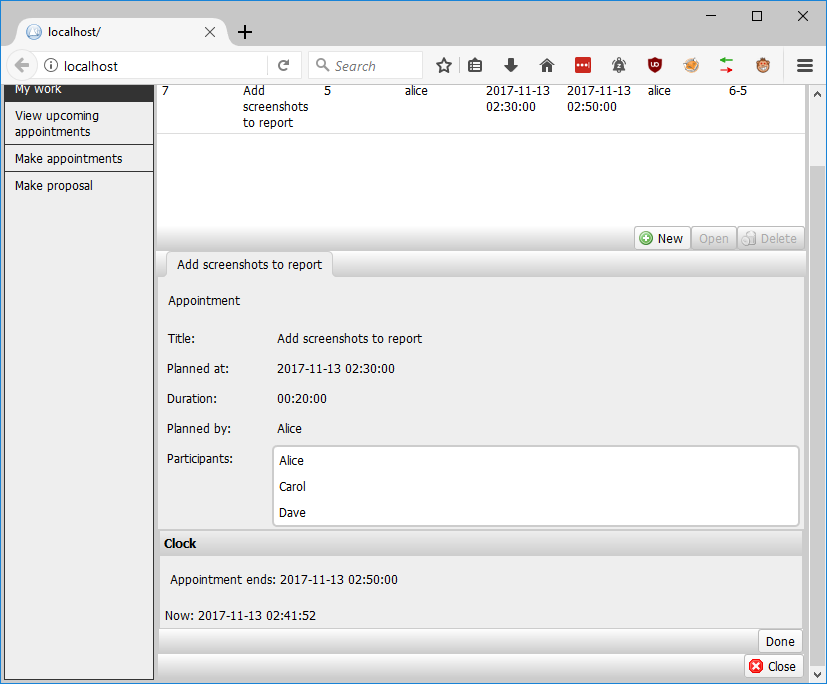
\includegraphics[width=\textwidth]{09_view_appointment}
		\caption{Viewing an active appointment}
	\end{figure}
	
	\begin{figure}[h!]
		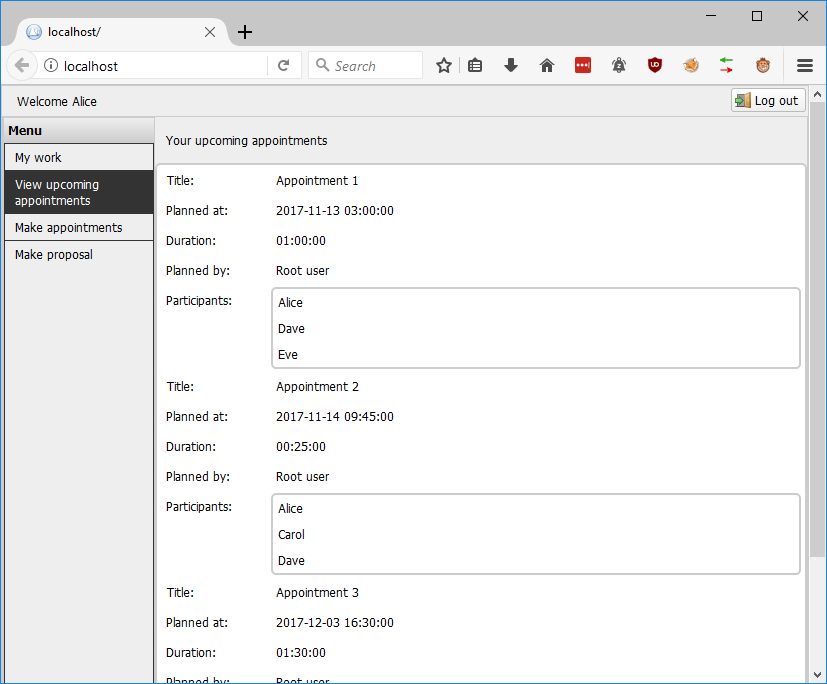
\includegraphics[width=\textwidth]{10_upcoming_appointments}
		\caption{Looking at upcoming appointments}
	\end{figure}
	
\end{document}
